\documentclass{beamer}
\usetheme[deutsch]{KIT}

\usepackage[utf8]{inputenc}
\usepackage[T1]{fontenc}
\usepackage{babel}
\usepackage{booktabs}
\usepackage{tikz,calc,ifthen}
\usepackage{mathtools}
\usepackage[normalem]{ulem}
\usepackage{graphicx}
\usepackage{xspace}
\usepackage{xcolor}
\usepackage{minted}
\usepackage{realboxes}
\usepackage{pifont}
\usepackage{stmaryrd}

\usetikzlibrary{positioning,calc,arrows,shapes}
\tikzset{
  every node/.style={transform shape},
  auto,
  block/.style={align=center,rectangle,draw,minimum height=20pt,minimum width=30pt},
  >=triangle 60,
  alt/.code args={<#1>#2#3}{%
      \alt<#1>{\pgfkeysalso{#2}}{\pgfkeysalso{#3}}
  },
  beameralert/.style={alt=<#1>{color=green!80!black}{}},
  mythick/.style={line width=1.4pt}
}

\newcommand*{\maxwidthofm}[2]{\maxof{\widthof{$#1$}}{\widthof{$#2$}}}
\newcommand<>*{\robustaltm}[2]{
  \alt#3
  {\mathmakebox[\maxwidthofm{#1}{#2}]{#1}\vphantom{#1#2}}
    {\mathmakebox[\maxwidthofm{#1}{#2}]{#2}\vphantom{#1#2}}
}

\newcommand<>*{\nodealert}[1]{\only#2{\draw[overlay,mythick,color=green!80!black] (#1.north west) rectangle (#1.south east)}}


%%% Typographic defs

% From https://stackoverflow.com/a/39363004/388010
% Add a period to the end of an abbreviation unless there's one
% already, then \xspace.
\makeatletter
\DeclareRobustCommand\onedot{\futurelet\@let@token\@onedot}
\def\@onedot{\ifx\@let@token.\else.\null\fi\xspace}

\def\eg{e.g\onedot} \def\Eg{E.g\onedot}
\def\ie{i.e\onedot} \def\Ie{I.e\onedot}
\def\cf{c.f\onedot} \def\Cf{C.f\onedot}
\def\etc{etc\onedot} \def\vs{vs\onedot}
\def\wrt{w.r.t\onedot} \def\dof{d.o.f\onedot}
\def\etal{et al\onedot}
\makeatother

\newcommand{\newdef}[1]{\emph{#1}}

\newcommand{\anal}[1]{\textsc{#1}\xspace}
\newcommand*{\MayAlias}{\anal{MayAlias}}
\newcommand*{\MustAlias}{\anal{MustAlias}}
\newcommand*{\MinCard}{\anal{MinCard}}
\newcommand*{\MaxCard}{\anal{MaxCard}}

%%% Minted for syntax highlighting

\newmintinline[hs]{haskell}{}
\newminted[haskell]{haskell}{linenos,mathescape,texcomments,autogobble}


\title{Call Arity vs. Demand Analysis}
\author{Sebastian Graf}
\subtitle{\insertauthor}
\institute[IPD]{Lehrstuhl Programmierparadigmen, IPD Snelting}
\date{9.8.2017}
\KITtitleimage{cover.png}

\begin{document}

\begin{frame}
  \maketitle
\end{frame}

\begin{frame}{Motivation}
  \begin{itemize}
    \item Glasgow Haskell Compiler (GHC): >100k lines of code
    \item Typical challenges of big software projects
    \item Two analyses with overlapping concerns
      \begin{itemize}
        \item Demand Analyser
        \item Call Arity
      \end{itemize}
    \item Extract overlaps into combined analysis
      \begin{itemize}
        \item Both prior analyses profit from increased precision
        \item Principle of DRY
      \end{itemize}
  \end{itemize}
\end{frame}

\begin{frame}[fragile]{Cardinality Analysis}
  \begin{itemize}
    \item 
      Provides lower and upper bounds on \emph{evaluation cardinality}
      \begin{itemize} \item \MinCard and \MaxCard analyses \end{itemize}
    \item Notation: $[n,m]$, where $n,m \in \{0,1,\omega\}, n \leq m$
  \end{itemize}
  \begin{center}
    \begin{minipage}{0.5\textwidth}
      \begin{haskell}
        main = do
          let a = ... -- $[1,\omega]$
              b = ... -- $[1,1]$
              c = ... -- $[0,\omega]$
              d = ... -- $[0,1]$
              e = ... -- $[0,0]$
          print (a + if b then a * d else c * c)
      \end{haskell}
    \end{minipage}
  \end{center}
\end{frame}

\begin{frame}[fragile]{Call-by-value}
  \begin{itemize}
    \item 
      Avoids operational complexity of laziness, enables unboxing
      \begin{itemize} \item Exploits \emph{strictness} \end{itemize}
      \begin{itemize} \item `Evaluated at \emph{least} once' (\MinCard) \end{itemize}
  \end{itemize}
  \begin{center}
    \begin{minipage}{0.5\textwidth}
      \begin{haskell}
        main = do
          let !a    = ...                 -- $[\mathbf{1},\omega]$
              !b    = ...                 -- $[\mathbf{1},1]$
               c    = ...                 -- $[0,\omega]$
               d    = ...                 -- $[0,1]$
               e    = ...                 -- $[0,0]$
          print (a + if b then a * d else c * c)
      \end{haskell}
    \end{minipage}
  \end{center}
\end{frame}

\begin{frame}[fragile]{Call-by-name}
  \begin{itemize}
    \item 
      Omits updates of \emph{single-entry} thunks, mimicing regular function calls
      \begin{itemize} \item Exploits lack of \emph{sharing} \end{itemize}
      \begin{itemize} \item `Evaluated at \emph{most} once' (\MaxCard) \end{itemize}
  \end{itemize}
  \begin{center}
    \begin{minipage}{0.5\textwidth}
      \begin{haskell}
        main = do
          let  a    = ...                 -- $[1,\omega]$
               b () = ...                 -- $[1,\mathbf{1}]$
               c    = ...                 -- $[0,\omega]$
               d () = ...                 -- $[0,\mathbf{1}]$
               e () = ...                 -- $[0,\mathbf{0}]$
          print (a + if b () then a * d () else c * c)
      \end{haskell}
    \end{minipage}
  \end{center}
\end{frame}

\begin{frame}[fragile]{Dead code}
  \begin{itemize}
    \item Can replace dead bindings with small traps
    \begin{itemize} \item Exploits \emph{absence} \end{itemize}
    \begin{itemize} \item `Never evaluated' (\MaxCard) \end{itemize}
  \end{itemize}
  \begin{center}
    \begin{minipage}{0.5\textwidth}
      \begin{haskell}
        main = do
          let  a    = ...                 -- $[1,\omega]$
               b    = ...                 -- $[1,1]$
               c    = ...                 -- $[0,\omega]$
               d    = ...                 -- $[0,1]$
               e    = error "e is absent" -- $[0,\mathbf{0}]$
          print (a + if b then a * d else c * c)
      \end{haskell}
    \end{minipage}
  \end{center}
\end{frame}

\begin{frame}[fragile]{Usage Analysis}
  \begin{itemize}
    \item \MaxCard analysis, \eg computes $m$ in binding annotations $[n,m]$
    \item 
      Related: \emph{one-shot} lambdas
  \end{itemize}
  \begin{center}
    \begin{minipage}{0.5\textwidth}
      \begin{haskell*}{escapeinside=||}
        main = do        
          let c = ...
              f = \|$\mathtt{x}^\omega$| |$\mathtt{y}^1$| -> c*x + y
              g = \|$\mathtt{z}^1$| -> 
                    let d = ... 
                    in \|$\mathtt{w}^1$| -> c*d + z*w
          print (f 1 2 + f 4 5 * g 3 42)
      \end{haskell*}
    \end{minipage}
  \end{center}
\end{frame}

% Proably backup, also useful to explain inlining
\begin{frame}[fragile]{Floating}
  \begin{itemize}
    \item Floating bindings in and out of expressions
    \item Floating into a lambda possibly duplicates work!
    \item Not so with one-shot lambdas
  \end{itemize}
  \begin{center}
    \begin{minipage}{0.5\textwidth}
      \begin{overprint}
        \onslide<1>
        \begin{haskell*}{escapeinside=||}
          main = do        
            let c = ...
                f = \|$\mathtt{x}^\omega$| |$\mathtt{y}^1$| -> c*x + y
                g = \|$\mathtt{z}^1$| -> 
                      let d = ... 
                      in \|$\mathtt{w}^1$| -> c*d + z*w
            print (f 1 2 + f 4 5 * g 3 42)
        \end{haskell*}
        \onslide<2>
        \begin{haskell*}{escapeinside=||}
          main = do        
            let |\color{red}\texttt{c}| = ...
                f = \|$\mathtt{x}^{\color{red} \omega}$| |$\mathtt{y}^1$| -> |\color{red}\texttt{c}|*x + y
                g = \|$\mathtt{z}^1$| -> 
                      let d = ... 
                      in \|$\mathtt{w}^1$| -> |\color{red}\texttt{c}|*d + z*w
            print (f 1 2 + f 4 5 * g 3 42)
        \end{haskell*}
        \onslide<3>
        \begin{haskell*}{escapeinside=||}
          main = do        
            let c = ...
                f = \|$\mathtt{x}^\omega$| |$\mathtt{y}^1$| -> c*x + y
                g = \|$\mathtt{z}^1$| -> 
                      let |\color{red}\texttt{d}| = ... 
                      in \|$\mathtt{w}^1$| -> c*|\color{red}\texttt{d}| + z*w
            print (f 1 2 + f 4 5 * g 3 42)
        \end{haskell*}
        \onslide<4>
        \begin{haskell*}{escapeinside=||}
          main = do        
            let c = ...
                f = \|$\mathtt{x}^\omega$| |$\mathtt{y}^1$| -> c*x + y
                g = \|$\mathtt{z}^1$| |$\mathtt{w}^1$| -> 
                      let |\color{red}\texttt{d}| = ... 
                      in c*|\color{red}\texttt{d}| + z*w
            print (f 1 2 + f 4 5 * g 3 42)
        \end{haskell*}
      \end{overprint}
    \end{minipage}
  \end{center}
\end{frame}

\begin{frame}[fragile]{$\eta$-Expansion}
  \begin{itemize}
    \item Floats lambdas out, possibly duplicating work
    \item Not so with one-shot lambdas
  \end{itemize}
  \begin{center}
    \begin{minipage}{0.5\textwidth}
      \begin{overprint}
        \onslide<1>
        \begin{haskell*}{escapeinside=||}
          main = do        
            let g = \|$\mathtt{z}^1$| -> 
                      let d = ... 
                      in \|$\mathtt{w}^{\color{red} 1}$| -> d + z*w
            print (g 3 42)
        \end{haskell*}
        \onslide<2>
        \begin{haskell*}{escapeinside=||}
          main = do        
            let g = \|$\mathtt{z}^1$| \|\color{red}$\mathtt{w}^1$| -> 
                      let d = ... 
                      in d + z*w
            print (g 3 42)
        \end{haskell*}
      \end{overprint}
    \end{minipage}
  \end{center}
\end{frame}

\begin{frame}[fragile]{Demand Analyser}
  \begin{overprint}
    \onslide<1>
    \begin{itemize}
      \item A cardinality analysis
      \item Usage analysis identifies
        \begin{itemize}
          \item Single-entry thunks
          \item One-shot lambdas
          \item Dead code
        \end{itemize}
      \item Computes how an expression uses its free variables
    \end{itemize}

    \onslide<2>
    \begin{itemize}
      \item Call Uses
        \begin{itemize}
          \item Identification of one-shot lambdas needs tracking of \emph{how} a binding was used
          \item Introduces \newdef{call uses} $C^n(u)$
          \item \hs{f 1 2} exposes \hs{f} to usage $1*C^1(C^1(U))$
          \item \hs{f 1 2 + f 4 5} exposes \hs{f} to usage $\omega*C^\omega(C^1(U))$
        \end{itemize}
    \end{itemize}
    \begin{center}
      \begin{minipage}{0.5\textwidth}
        \begin{haskell*}{escapeinside=||}
          let f |$\mathtt{x}^\omega$| |$\mathtt{y}^1$| = ...
          in f 1 2 + f 4 5
        \end{haskell*}
      \end{minipage}
    \end{center}

    \onslide<3>
    \begin{itemize}
      \item Usage Signatures
        \begin{itemize}
          \item Interprocedural data-flow
          \item \hs{const} has \newdef{usage signature} $1*U \to A \to \bullet$
          \item \hs{y} is used once, $1*U$
          \item \hs{fac 1000} is dead code ($A$ for absent, \eg never used)
          \item Usage signature + free variable usage = \newdef{usage type}
          \item Looks at the definition of \hs{const} before the \hs{let} body!
            \begin{itemize} 
              \item \textsc{LetDn} rule: Unleashes usage types of \hs{const} at call sites
            \end{itemize}
        \end{itemize}
    \end{itemize}
    \begin{center}
      \begin{minipage}{0.5\textwidth}
        \begin{haskell*}{escapeinside=||}
          let const a b = a
          in const y (fac 1000)
        \end{haskell*}
      \end{minipage}
    \end{center}

    \onslide<4>
    \begin{itemize}
      \item Thunks
        \begin{itemize}
          \item \hs{x} is only used once, its evaluation in \hs{y}'s right-hand side is shared!
          \item 
            Two use sites 
            \begin{itemize} 
              \item \textsc{LetDn}-style leads to usage of $\omega*U$ on \hs{x}! 
            \end{itemize}
          \item Solution: \textsc{LetUp} for thunks
            \begin{itemize} 
              \item Record usage $\omega*U$ of \hs{y} in the body of the \hs{let}
              \item Analyse \hs{y}'s bound expression in use $U$, unleash its usage type
            \end{itemize}
        \end{itemize}
    \end{itemize}
    \begin{center}
      \begin{minipage}{0.5\textwidth}
        \begin{haskell*}{escapeinside=||}
          let y = 2*x
          in y + y
        \end{haskell*}
      \end{minipage}
    \end{center}
 \end{overprint}
\end{frame}

\begin{frame}[fragile]{Call Arity}
  \begin{overprint}
    \onslide<1>
    \begin{itemize}
      \item $\eta$-expansion based on usage information
      \item \hs{f} is always called with two arguments
      \item<2> \hs{f}'s bound expression can be $\eta$-expanded!
    \end{itemize}
    \begin{center}
      \begin{minipage}{0.5\textwidth}
        \begin{haskell}
          let f x = 
                if expensive
                then id
                else (*x)
          in f 1 2 + f 4 5
        \end{haskell}
      \end{minipage}
    \end{center}

    \onslide<2>
    \begin{itemize}
      \item $\eta$-expansion based on usage information
      \item \hs{f} is always called with two arguments
      \item<2> \hs{f}'s bound expression can be $\eta$-expanded!
    \end{itemize}
    \begin{center}
      \begin{minipage}{0.5\textwidth}
        \begin{haskell}
          let f x y = 
                if expensive
                then y
                else y*x
          in f 1 2 + f 4 5
        \end{haskell}
      \end{minipage}
    \end{center}

    \onslide<3>
    \begin{itemize}
      \item Can we $\eta$-expand \hs{f} here?
      \item \hs{f} is always called with two arguments
      \item<4> ... but \hs{f} is also a thunk! 
      \item<4> $\eta$-expansion would duplicate the \hs{expensive} check!
    \end{itemize}
    \begin{center}
      \begin{minipage}{0.5\textwidth}
        \begin{haskell}
          let f = 
                if expensive
                then \x y -> y
                else \x y -> y*x
          in f 1 2 + f 4 5
        \end{haskell}
      \end{minipage}
    \end{center}

    \onslide<4>
    \begin{itemize}
      \item Can we $\eta$-expand \hs{f} here?
      \item \hs{f} is always called with two arguments
      \item<4> ... but \hs{f} is also a thunk
      \item<4> $\eta$-expansion would duplicate the \hs{expensive} check!
    \end{itemize}
    \begin{center}
      \begin{minipage}{0.5\textwidth}
        \begin{haskell}
          let f = 
                if expensive
                then \x y -> y
                else \x y -> y*x
          in f 1 2 + f 4 5
        \end{haskell}
      \end{minipage}
    \end{center}

    \onslide<5>
    \begin{itemize}
      \item Can we $\eta$-expand \hs{f} here?
      \item \hs{f} is a thunk, called with two arguments
      \item<6> Since \hs{f} is \emph{called} only \emph{once}, $\eta$-expansion is safe
    \end{itemize}
    \begin{center}
      \begin{minipage}{0.5\textwidth}
        \begin{haskell}
          let f = 
                if expensive
                then \x y -> y
                else \x y -> y*x
          in if b then f 1 2 else f 4 5
        \end{haskell}
      \end{minipage}
    \end{center}

    \onslide<6>
    \begin{itemize}
      \item Can we $\eta$-expand \hs{f} here?
      \item \hs{f} is a thunk, called with two arguments
      \item<6> Since \hs{f} is only \emph{called once}, $\eta$-expansion is safe
      % Also demnostrates why we can't generally just inline \hs{f}
    \end{itemize}
    \begin{center}
      \begin{minipage}{0.5\textwidth}
        \begin{haskell}
          let f x y = 
                if expensive
                then y
                else y*x
          in if b then f 1 2 else f 4 5
        \end{haskell}
      \end{minipage}
    \end{center}

    \onslide<7>
    \begin{itemize}
      \item Called-once information is tracked by a usage analysis
      \item Analyses \hs{let} body before bound expression, bottom-up, like \textsc{LetUp}
      \item Ordinary \textsc{LetUp}-style usage analysis too imprecise
        \begin{itemize}
          \item Forgets that \hs{x} and \hs{y} were evaluated on different code paths
          \item Analysis reports \hs{x} to be used multiple times
        \end{itemize}
    \end{itemize}
    \begin{center}
      \begin{minipage}{0.5\textwidth}
        \begin{haskell}
          let x = ...  
          in let y = 2*x
             in if b
                then x
                else y
        \end{haskell}
      \end{minipage}
    \end{center}

    \onslide<8>
    \begin{itemize}
      \item \emph{Co-call graphs} track control flow information
        \begin{itemize}
          \item Edges connect variables possible evaluated on the same code path
          \item Absence of an edge proves mutual exclusive calls
          \item Usage information in self-edges
        \end{itemize}
      \item Lack of edge between \hs{x} and \hs{y} avoids self-edge on \hs{x}
    \end{itemize}
    \begin{columns}
      \begin{column}{0\textwidth}
        \begin{haskell}
          let x = ...  
          in let y = 2*x
             in if b
                then x
                else y
        \end{haskell}
      \end{column}
      \begin{column}{0\textwidth}
        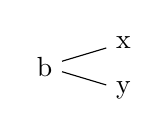
\begin{tikzpicture}
          \node at (0,0) (0) {\hs{b}};
          \node at (1,0.3) (1) {\hs{x}};
          \node at (1,-0.3) (2) {\hs{y}};
          \draw (0) -- (1);
          \draw (0) -- (2);
        \end{tikzpicture}
      \end{column}
    \end{columns}

    \onslide<9>
    \begin{itemize}
      \item \emph{Co-call graphs} track control flow information
        \begin{itemize}
          \item Edges connect variables possible evaluated on the same code path
          \item Absence of an edge proves mutual exclusive calls
          \item Usage information in self-edges
        \end{itemize}
      \item Lack of edge between \hs{x} and \hs{y} avoids self-edge on \hs{x}
    \end{itemize}
    \begin{columns}
      \begin{column}{0\textwidth}
        \begin{haskell}
          let x = ...  
          in let y = 2*x
             in if b
                then x
                else y
        \end{haskell}
      \end{column}
      \begin{column}{0\textwidth}
        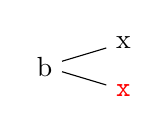
\begin{tikzpicture}
          \node at (0,0) (0) {\hs{b}};
          \node at (1,0.3) (1) {\hs{x}};
          \node at (1,-0.3) (2) {\color{red}\texttt{x}};
          \draw (0) -- (1);
          \draw (0) -- (2);
        \end{tikzpicture}
      \end{column}
    \end{columns}

    \onslide<10>
    \begin{itemize}
      \item \emph{Co-call graphs} track control flow information
        \begin{itemize}
          \item Edges connect variables possible evaluated on the same code path
          \item Absence of an edge proves mutual exclusive uses
          \item Usage information in self-edges
        \end{itemize}
      \item Lack of edge between \hs{x} and \hs{y} avoids self-edge on \hs{x}
    \end{itemize}
    \begin{columns}
      \begin{column}{0\textwidth}
        \begin{haskell}
          let x = ...  
          in let y = 2*x
             in if b
                then x
                else y
        \end{haskell}
      \end{column}
      \begin{column}{0\textwidth}
        \begin{tikzpicture}
          \node at (0,0) (0) {\hs{b}};
          \node at (1,0) (1) {\hs{x}};
          \draw (0) -- (1);
        \end{tikzpicture}
      \end{column}
    \end{columns}
  \end{overprint}
\end{frame}

\begin{frame}{Combined Usage Analysis}
  \begin{itemize}
    \item Idea: Extend usage analysis of the Demand Analyser
    \item Add co-call graphs to usage types for tracking single-entry thunks
    \item Glorified \textsc{LetDn}-style analysis with precise call uses for functions
  \end{itemize}
\end{frame}

\begin{frame}[fragile]{Call Arity vs. Demand Analysis}
  \begin{overprint}
    \onslide<1>
    \begin{itemize}
      \item Free variable \hs{z} is used only once
      \item Recall: Demand Analysis unleashes function bindings top-down (\textsc{LetDn})
      \item \textsc{LetDn} only digests \hs{f} for manifest arity 1, can't look under lambda
      \item \hs{f} is called with 2 arguments, $C^1(C^1(U))$
      \item[\xmark] Demand Analysis: \hs{z} is annotated as used multiple times
      \item[\cmark] Call Arity (\textsc{LetUp}): Arity information flows bottom-up, \hs{z} used once
    \end{itemize}
    \begin{center}
      \begin{minipage}{0.5\textwidth}
        \begin{haskell*}{escapeinside=||}
          let f x = 
                if expensive
                then \y -> y*|\color{red}\texttt{z}|
                else \y -> y*x
          in f 1 2
        \end{haskell*}
      \end{minipage}
    \end{center}

    \onslide<2>
    \begin{itemize}
      \item[\xmark] Demand Analysis: \hs{z} is annotated as used multiple times
      \item[\cmark] Call Arity (\textsc{LetUp}): Arity information flows bottom-up, \hs{z} used once
      \item Solution: Analyse bound function on demand, when we know specific call use 
    \end{itemize}
    \begin{center}
      \begin{minipage}{0.5\textwidth}
        \begin{haskell*}{escapeinside=||}
          let f x = 
                if expensive
                then \y -> y*|\color{red}\texttt{z}|
                else \y -> y*x
          in f 1 2
        \end{haskell*}
      \end{minipage}
    \end{center}
  \end{overprint}
\end{frame}

\begin{frame}[fragile]{Combined Usage Analysis}
  \begin{itemize}
    \item Glorified \textsc{LetDn}-style analysis with precise call uses for functions
      \begin{itemize} \item Analyse bound function on demand, when we know specific call use \end{itemize}
    \item Recursion leads to termination problems
    \item Rediscovered fixed-point iteration, detached from the syntax tree
    \item Led to graph-based abstraction solved by worklist algorithm
  \end{itemize}
  \begin{center}
    \begin{minipage}{0.5\textwidth}
      \begin{haskell}
        let fac n = 
              if n == 0
              then 1
              else n * fac (n-1)
        in fac 12
      \end{haskell}
    \end{minipage}
  \end{center}
\end{frame}

\begin{frame}{Transfer Function}
  \begin{itemize}
    \item Specification denotes expressions by (monotone) \newdef{usage transformers}
    \item $\sUTrans = \sUse \to \sUType$
    \item Reflects dependency on incoming use (\eg arity)
    \item $\transfer{\uscore}{\uscore[\rho]} : \sExp \to \sTransEnv \to \sUTrans$
  \end{itemize}
  \begin{alignat*}{2}
    \transfer{\sLet{\bind}{e}}{\rho}\,u &{}={}&& (\cmblet{\theta}{\maplit{x_1}{\theta_1}}) \setminus_{x_1} \\
    \text{where} \\
     \tau_1 &{}={}&& \transfer{e_1}{\rho} \\
     \rho' &{}={}&& \maplit{x_1}{\letdown{\tau_1}{e_1}}\rho \\ 
     \theta &{}={}&& \transfer{e}{\rho'}\,u \\ 
     \theta_1 &{}={}&& \liftqm{\letup{\tau_1}{e_1}}{\theta(x_1)}
  \end{alignat*}
\end{frame}

\begin{frame}[fragile]{Recovering Call Arity}
  \begin{itemize}
    \item Observation: (Safe) $\eta$-expansion does not change how an expression is used
    \item Perform $\eta$-Expansion based on Usage results $n*u$
  \end{itemize}
  \begin{overprint}
    \onslide<1>
    \[
      \begin{array}{lcl}
        \expand_{\sUsage}                              &\,\colon& \sUsage \to \mathbb{N} \to \mathbb{N} \\
        \expand_{\sUsage}\,A\,\alpha                   &    =   & \alpha \\
        \expand_{\sUsage}\,(\omega*\uscore[u])\,0      &    =   & 0 \\
        \expand_{\sUsage}\,(\uscore[\omega]*u)\,\alpha &    =   & \expand_{\sUse}\,u\,\alpha \\
        \\
        \expand_{\sUse}                                &\,\colon& \sUse \to \mathbb{N} \to \mathbb{N} \\
        \expand_{\sUse}\,C^\omega(u)\,0                &    =   & 0 \\
        \expand_{\sUse}\,C^{\uscore}(u)\,\alpha        &    =   & 1 + \expand_{\sUsage}\,u\,(\max\,0\,(\alpha - 1)) \\
        \expand_{\sUse}\,\uscore\,\alpha               &    =   & \alpha \\
      \end{array}
    \]

    \onslide<2>
    \begin{center}
      \begin{minipage}[t][10cm][t]{0.5\textwidth}
        \begin{haskell}
          let f x =   -- $\omega*C^\omega(C^{\color{red} 1}(U))$
                if b
                then \y -> y
                else \y -> y*x
          in f 1 2 + f 4 5
        \end{haskell}
      \end{minipage}
    \end{center}

    \onslide<3>
    \begin{center}
      \begin{minipage}{0.5\textwidth}
        \begin{haskell*}{escapeinside=||}
          let f x |\color{mygreen}\texttt{y}| = -- $\omega*C^\omega(C^1(U))$
                if b
                then y
                else y*x
          in f 1 2 + f 4 5
        \end{haskell*}
      \end{minipage}
    \end{center}

    \onslide<4>
    \begin{center}
      \begin{minipage}{0.5\textwidth}
        \begin{haskell}
          let t =     -- ${\color{red} \omega}*C^\omega(C^1(U))$
                if b
                then \x y -> y
                else \x y -> y*x 
          in t 1 2 + t1 4 5
        \end{haskell}
      \end{minipage}
    \end{center}

    \onslide<5>
    \begin{center}
      \begin{minipage}{0.5\textwidth}
        \begin{haskell}
          let t =     -- ${\color{red} 1}*C^1(C^1(U))$
                if b
                then \x y -> y
                else \x y -> y*x 
          in t 1 2
        \end{haskell}
      \end{minipage}
    \end{center}

    \onslide<6>
    \begin{center}
      \begin{minipage}{0.5\textwidth}
        \begin{haskell}
          let t =     -- $1*C^{\color{red} 1}(C^1(U))$
                if b
                then \x y -> y
                else \x y -> y*x 
          in t 1 2
        \end{haskell}
      \end{minipage}
    \end{center}

    \onslide<7>
    \begin{center}
      \begin{minipage}{0.5\textwidth}
        \begin{haskell*}{escapeinside=||}
          let t |\color{mygreen}\texttt{x}| =   -- $1*C^1(C^{\color{red} 1}(U))$
                if b
                then \y -> y
                else \y -> y*x 
          in t 1 2
        \end{haskell*}
      \end{minipage}
    \end{center}

    \onslide<8>
    \begin{center}
      \begin{minipage}{0.5\textwidth}
        \begin{haskell*}{escapeinside=||}
          let t x |\color{mygreen}\texttt{y}| = -- $1*C^1(C^1(U))$
                if b
                then y
                else y*x
          in t 1 2
        \end{haskell*}
      \end{minipage}
    \end{center}
  \end{overprint}
\end{frame}

\begin{frame}[fragile]{Implementation}
  \begin{itemize}
    \item Central part of GHC, changes with many repercussions
    \item Co-call graphs: Efficient representation of sparse and dense cases
    \item Solving the data-flow problem through graph-based fixed-point iteration
    \item Montonicity issues due to a lack of appropriate data structures for monotone maps
  \end{itemize}
\end{frame}

\begin{frame}[fragile]{Evaluation}
  \begin{overprint}
    \onslide<1>
    \begin{itemize}
      \item Benchmarked two variants, baseline GHC 8.2.1
        \begin{itemize}
          \item Full analysis, with co-call graphs
          \item Without co-call graphs, but with glorified \textsc{LetDn}
        \end{itemize}
      \item Measured allocations and executed instructions
        \begin{itemize}
          \item Artifact performance on nofib suite
          \item Compiler performance compiling nofib and stage2 compiler
        \end{itemize}
    \end{itemize}

    \onslide<2>
    \begin{columns}
      \begin{column}{0.4\textwidth}
        \begin{itemize}
          \item No regressions relative to the baseline (technically)
          \item Co-call graphs didn't influence allocations noticeably
        \end{itemize}
      \end{column}
      \begin{column}{0.6\textwidth}
        \begin{table}
          \centering
          \begin{tabular}{lrr}
            \toprule
                    & \multicolumn{2}{c}{Bytes allocated} \\
                      \cmidrule(lr){2-3}
            Program & \multicolumn{1}{c}{\varfull} & \multicolumn{1}{c}{\varedges} \\
            \midrule
            \progname{fft2} & -0.9\% & -0.9\%\\
\progname{fluid} & -1.5\% & -1.5\%\\
\progname{infer} & +0.0\% & +0.0\%\\
\progname{n-body} & -0.2\% & -0.2\%\\
\progname{tak} & -0.4\% & -0.4\%\\
\andmore{98} & & \\
\midrule
\totalname{Min} & -1.5\% & -1.5\%\\
\totalname{Max} & +0.0\% & +0.0\%\\
\totalname{Geometric Mean} & -0.0\% & -0.0\%\\



            \bottomrule
          \end{tabular}
        \end{table}
      \end{column}
    \end{columns}

    \onslide<3>
    \begin{columns}
      \begin{column}{0.4\textwidth}
        \begin{itemize}
          \item Wild outliers, unclear why
          \item Plays out in our favour
          \item Co-call graphs make a slight difference
        \end{itemize}
      \end{column}
      \begin{column}{0.6\textwidth}
        \begin{table}
          \centering
          \begin{tabular}{lrr}
            \toprule
                    & \multicolumn{2}{c}{Instructions executed} \\
                      \cmidrule(lr){2-3}
            Program & \multicolumn{1}{c}{\varfull} & \multicolumn{1}{c}{\varedges} \\
            \midrule
            \progname{fannkuch-redux} & +11.4\% & +11.4\% & +11.4\%\\
\progname{gen\_regexps} & -28.1\% & -28.1\% & -28.1\%\\
\progname{maillist} & -0.2\% & +2.1\% & +3.4\%\\
\progname{paraffins} & -3.4\% & -3.4\% & -3.4\%\\
\progname{puzzle} & -15.4\% & -15.4\% & -15.4\%\\
\progname{sphere} & -4.5\% & -4.4\% & -4.4\%\\
\andmore{97} & & & \\
\midrule
\totalname{Min} & -28.1\% & -28.1\% & -28.1\%\\
\totalname{Max} & +11.4\% & +11.4\% & +11.4\%\\
\totalname{Geometric Mean} & -0.6\% & -0.6\% & -0.6\%\\



            \bottomrule
          \end{tabular}
        \end{table}
      \end{column}
    \end{columns}

    \onslide<4>
    \begin{itemize}
      \item Compiler performance got worse
        \begin{itemize}
          \item One run of Call Arity replaced by three runs of our usage analysis
        \end{itemize}
      \item GHC stage2 compiler built without optimisations
      \item Space usage of variant \varfull goes through the roof
    \end{itemize}
    \begin{table}
      \centering
      \begin{tabular}{lrrrr}
        \toprule
                & \multicolumn{2}{c}{Bytes allocated} & \multicolumn{2}{c}{Instructions executed} \\
                  \cmidrule(lr){2-3} \cmidrule(lr){4-5}
        Program & \multicolumn{1}{c}{\varfull} & \multicolumn{1}{c}{\varedges} & \multicolumn{1}{c}{\varfull} & \multicolumn{1}{c}{\varedges} \\
        \midrule
        \totalname{nofib} & +29.8\% & +26.9\% & +11.0\% & +27.5\% & +24.5\% & +11.3\%\\

        \totalname{ghc} & +2.4\% & +2.3\% & +1.5\% & +2.3\% & +1.6\% & +1.1\% \\

        \bottomrule
      \end{tabular}
    \end{table}
  \end{overprint}
\end{frame}

\begin{frame}{Conclusion}
  \begin{itemize}
    \item Usage analysis generalising Call Arity and its counterpart in the Demand Analyser
      \begin{itemize}
        \item No regressions, but no real improvement either
      \end{itemize}
    \item 
      \texttt{\$ git diff --shortstat ghc-8.2.1-release cocall-full}\\
      \texttt{52 files changed, 3012 insertions(+), 1053 deletions(-)}
    \item Future work
      \begin{itemize}
        \item `Novel' approach to fixed-point iteration, detached from syntax tree
        \item Data structure for monotone maps
        \item Long term: Integration into GHC
      \end{itemize}
  \end{itemize}
\end{frame}

\end{document}
